\section{The Homotopy Form of Cauchy's Theorem}

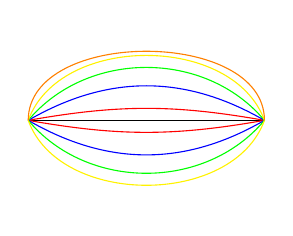
\begin{tikzpicture}
    \coordinate (O) at (0,0,0);
    \coordinate (A) at (3,0,0);
  
    \draw[] (O)--(A);
    \draw[color=red] (O) to [bend left=10] (A);
    \draw[color=red] (O) to [bend right=10] (A);
    \draw[color=blue] (O) to [bend left=30] (A);
    \draw[color=blue] (O) to [bend right=30] (A);
    \draw[color=green] (O) to [bend left=50] (A);
    \draw[color=green] (O) to [bend right=50] (A);
    \draw[color=yellow] (O) to [bend left=70] (A);
    \draw[color=yellow] (O) to [bend right=70] (A);
    \draw[color=orange] (O) to [bend left=90] (A);
  \end{tikzpicture}
